\documentclass[tikz,border=10pt]{standalone}
\begin{document}
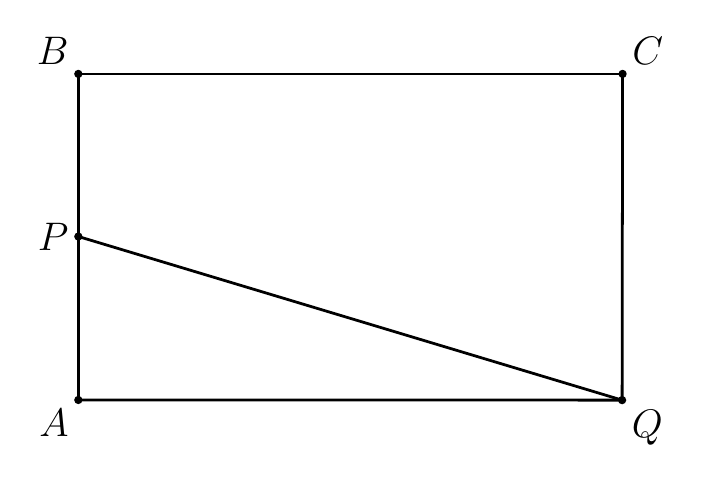
\begin{tikzpicture}[line join=round]
\coordinate (A) at (-3.465,-2.009);
\coordinate (B) at (-3.465,2.132);
\coordinate (C) at (3.447,2.132);
\coordinate (P) at (-3.465,0.067);
\coordinate (Q) at (3.441,-2.011);

  

  
  \draw[solid, line width=1.0pt] (B) -- (C);   
  \draw[solid, line width=1.0pt] (C) -- (Q);   
  \draw[solid, line width=1.0pt] (A) -- (Q);   
  \draw[solid, line width=1.0pt] (B) -- (P);   
  \draw[solid, line width=1.0pt] (P) -- (A);   
  \draw[solid, line width=1.0pt] (P) -- (Q);   

  
  \foreach \v in {A,B,C,P,Q} \fill (\v) circle (1.500pt);

  
  \node[above left]  at (B) {\fontsize{14.5}{17.4}\selectfont $B$};
  \node[above right] at (C) {\fontsize{14.5}{17.4}\selectfont $C$};
  \node[below left]  at (A) {\fontsize{14.5}{17.4}\selectfont $A$};
  \node[below right] at (Q) {\fontsize{14.5}{17.4}\selectfont $Q$};
  \node[left]        at (P) {\fontsize{14.5}{17.4}\selectfont $P$};
\end{tikzpicture}
\end{document}